\section{Beam diagnostic and IPM}
\subsection{Beam diagnostic at ESS}
\begin{frame}
  \frametitle{Beam diagnostic at ESS}
  \begin{block}{ESS is based on a power accelerator}
    Beam diagnostics are mandatory tools to insure safety and acquire knowledge about the beam:
    \begin{itemize}
      \item 15 different systems: Beam position, beam current, beam energy, beam losses ...
      \item A total of 480 beam diagnostics along the accelerator.
      \item Various fields are involved in the development of these devices.
    \end{itemize}
  \end{block}

  Today, we are presenting a device that measure the \textbf{transverse beam profile}:
  \begin{columns}
    \begin{column}{0.60\textwidth}
      \begin{block}{Definition}
        Spacial distribution of the charges of the beam in the transverse plane.
        \begin{itemize}
          \item Beam shape
          \item Beam position
          \item Relative beam amplitude
        \end{itemize}
      \end{block}
    \end{column}
    \begin{column}{0.30\textwidth}
      \centering
      \includegraphics[width=0.5\textwidth]{02_ESS/fig/fig000_profile2}
    \end{column}
  \end{columns}
\end{frame}

% \begin{frame}
%   \frametitle{Profile measurement method}
%   \includegraphics[width=\textwidth]{01_Neutron/fig/fig000_ESS_acc}
%   \begin{columns}
%     \begin{column}{0.45\textwidth}
%       \begin{block}{Wire Scanner/SEM Grid}
%         Measurement of the secondaries electrons or hadronic cascade emitted during the collision of proton with one or more wires.
%       \end{block}
%       \begin{block}{Pros/cons}
%         \begin{itemize}
%           \item[+] High sensitivity
%           \item[-] Interceptive measurement
%         \end{itemize}
%       \end{block}
%     \end{column}
%     \begin{column}{0.45\textwidth}
%       Image/Schema
%       \begin{block}{Use at ESS}
%         \begin{itemize}
%           \item Everywhere along accelerator
%           \item But limited to low duty cycle
%         \end{itemize}
%       \end{block}
%     \end{column}
%   \end{columns}
%   \begin{alertblock}{Wire scanners cannot work at nominal conditions}
%     The WS can not withstand the $5\,\mathrm{MW}$ beam power. Wire can melt and may compromise the SC cavities.
%   \end{alertblock}
% \end{frame}

\subsection{Profile measurement method at ESS}
\begin{frame}
  \frametitle{Profile measurement method}
  \includegraphics[width=\textwidth]{01_Neutron/fig/fig000_ESS_acc}
  \begin{columns}
    \begin{column}{0.45\textwidth}
      \begin{block}{Fluorescence \textbf{Profile Monitor} (FPM)}
        Measurement of the fluorescence induced by the beam.
      \end{block}
      \begin{block}{Pros/cons}
        \begin{itemize}
          \item[+] Non-invasive
          \item[+] No active elements in vacuum
          \item[-] $4\pi$ solid angle
          \item[-] Depends on vacuum
        \end{itemize}
      \end{block}
    \end{column}
    \begin{column}{0.45\textwidth}
      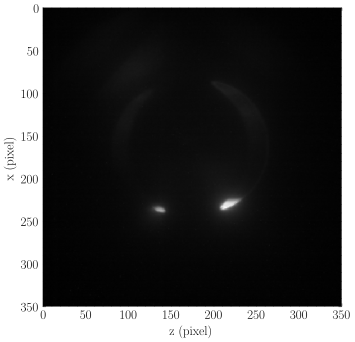
\includegraphics[width=\textwidth]{02_ESS/fig/fig000_FPM}

      \begin{block}{Use at ESS}
        \begin{itemize}
          \item In the warm parts of the accelerator
        \end{itemize}
      \end{block}
    \end{column}
  \end{columns}
  \begin{alertblock}{FPM cannot work in superconducing part}
    In the cryogenic section, the pressure is too low for FPM (expected $10^{-9}\,\mathrm{mbar}$).
  \end{alertblock}
\end{frame}

\begin{frame}
  \frametitle{Ionization Profile Monitor}
  \begin{alertblock}{So no profile measurement in SC part at nominal condition?}
    The measurement can be done by using an Ionization \textbf{Profile Monitor} (IPM).
  \end{alertblock}

  \begin{columns}
    \begin{column}{0.45\textwidth}
      \begin{block}{How it works}
        \begin{enumerate}
          \item Beam protons pass through the residual gas, inducing ionizations: $e^-$/ion pairs.
          \item An electric field drives $e^-$ or ions towards a segmented readout system.
          \item Profile in one transverse direction. Complete profile: pair of IPMs.
        \end{enumerate}
      \end{block}
    \end{column}
    \begin{column}{0.45\textwidth}
      \centering
      \includegraphics[width=0.8\textwidth]{02_ESS/fig/fig000_IPM.pdf}
    \end{column}
  \end{columns}
\end{frame}

\begin{frame}
  \frametitle{IPM}
  \begin{columns}[T]
    \begin{column}{0.45\textwidth}
      \begin{block}{Pros/cons}
        \begin{itemize}
          \item[+] Direct collection
          \item[+] Non invasive method
          \item[-] Vacuum dependant
          \item[-] Complex and expansive design (frame, HV, readout in vacuum)
          \item[-] Profile distortion
        \end{itemize}
      \end{block}

    \end{column}
    \begin{column}{0.45\textwidth}
      \begin{block}{History}
        \begin{itemize}
          \item 1960-1970: First use of an IPM.
          \item 1990-2000: Development of MCPs.
          \item 2015: Interest in semiconductor (CERN).
          \item Improvement of electronics and simulation capabilities.
        \end{itemize}
      \end{block}
    \end{column}
  \end{columns}


  IPMs are popular on proton circular accelerators or storage rings:
  \begin{itemize}
    \item Where vacuum can be extremely low (below $10^{-10}\,\mathrm{mbar}$)
    \item Pulse passes several times in the IPM
  \end{itemize}
  IPMs become popular for high intensity superconducting LINAC.
\end{frame}

\subsection{Project overview}
\begin{frame}
  \frametitle{Project overview}
  \begin{alertblock}{Subject of the thesis:}
    \textbf{Can we use IPMs in the superconducting part of the ESS accelerator?}
  \end{alertblock}
  \begin{block}{Project in brief}
    Provide 5 pairs of IPMs for the superconducting part of the ESS accelerator.

    Project milestones:
    \begin{itemize}
      \item[2016] Kick-off meeting (April), beginning of my PhD (October)
      \item[2017] Preliminary Design Review (February), \textbf{simulations, design and manufacturing}
      \item[2018] \textbf{Mainly beam tests and data analysis}
      \item[2019] Critical Design Review (March), design and manufacturing of final IPMs, end of my PhD (October)
      \item[2020] First IPM delivery, Handover
    \end{itemize}
  \end{block}
\end{frame}